\chapter{HASIL DAN PEMBAHASAN}
\label{chap:hasilpembahasan}

% Ubah bagian-bagian berikut dengan isi dari pengujian dan analisis

% Pada penelitian ini dipaparkan \lipsum[1][1-5]

\section{Hasil Penelitian}
\label{sec:hasil penelitian}
Sistem yang sudah dibuat mampu memenuhi batasan-batasan yang telah ditentukan \linebreak sebelumnya dan individu terbaik dapat menghasilkan nilai fitness 1.00. Nilai fitness 1.00 \linebreak berarti tidak ada batasan yang dilanggar. Contoh hasil keluaran program penjadwalan otomatis ini adalah sebagai berikut:
 
\begin{lstlisting}[language=Python,caption={Output penjadwalan otomatis}]
  Generation:  105831
  3
  Mutate
  Fitness a: 1.0
  Fitness b: 1.0
  Chromosome terbaik: 
  [[10, 2, 3, 1], [9, 26, 4, 1], [17, 9, 5, 1], [11, 5, 2, 3], [7, 18, 3, 3], [6, 12, 5, 3], [10, 25, 3, 4], [15, 32, 4, 4], [12, 28, 5, 4], [2, 35, 2, 5], [3, 16, 4, 5], [9, 10, 6, 5], [9, 6, 7, 6], [14, 1, 1, 6], [17, 14, 3, 6], [2, 4, 2, 6], [10, 27, 4, 6], [13, 37, 1, 7], [4, 33, 7, 7], [5, 22, 5, 7], [1, 11, 4, 7], [11, 21, 2, 8], [7, 13, 4, 8], [3, 30, 7, 8], [2, 24, 5, 9], [9, 29, 4, 10], [17, 20, 4, 11], [5, 7, 6, 11], [16, 17, 3, 12], [11, 38, 6, 12], [4, 3, 5, 12], [2, 8, 4, 12], [6, 15, 4, 13], [11, 34, 2, 14], [3, 36, 4, 14], [14, 31, 7, 14], [13, 19, 6, 14], [2, 23, 3, 14]]
\end{lstlisting}
\begin{figure} [ht] \centering
  % Nama dari file gambar yang diinputkan
  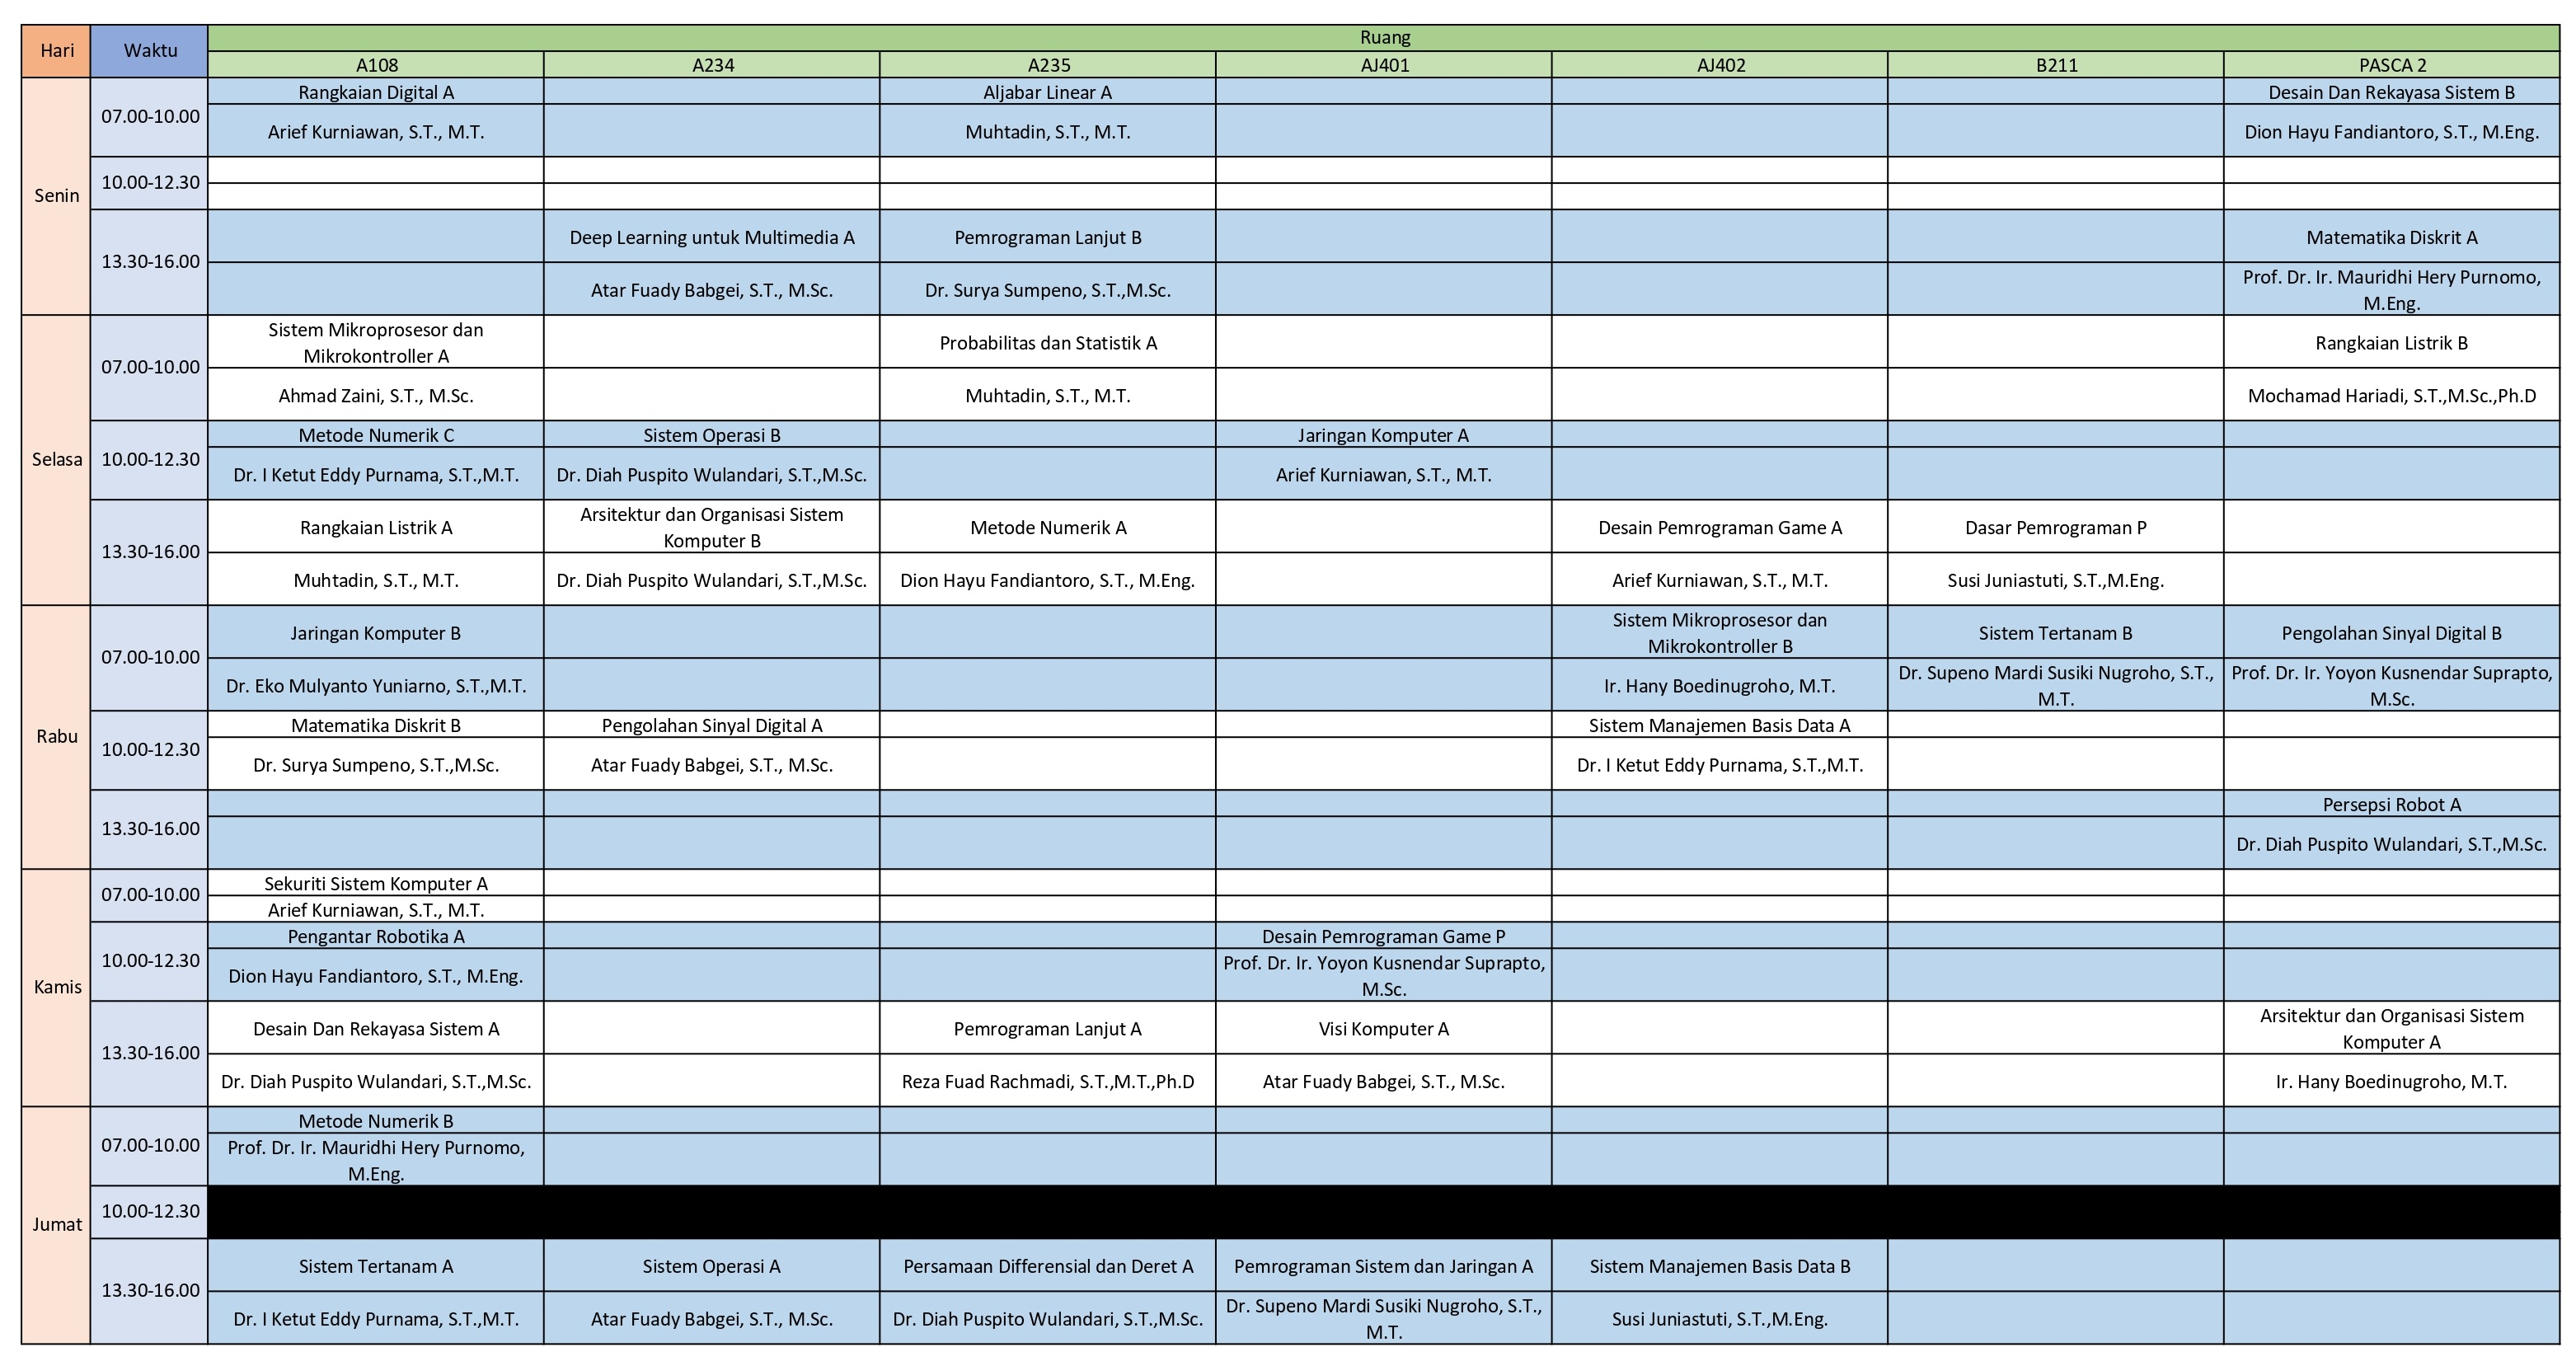
\includegraphics[scale=0.6]{gambar/jadwal.jpg}
  % Keterangan gambar yang diinputkan
  \caption{Jadwal Perkuliahan dari Kromosom Terbaik}
  % Label referensi dari gambar yang diinputkan
  \label{fig:jadwal}
\end{figure}
Hasil keluaran program diatas merupakan hasil keluaran dari percobaan penjadwalan otomatis yang memperhatikan kapasitas ruangan dan jumlah peserta tiap mata kuliah dan menggunakan probabilitasan percobaan yang memperhatikan probabilitasis mutasi sebesar 0.05. Percobaan ini memakan waktu 14 menit 52 detik.

Terdapat dua percobaan yang dilakukan dalam sistem penjadwalan otomatis ini. Percobaan pertama yaitu tanpa memperhatikan kapasitas kelas dan jumlah perserta tiap mata kuliah, dan percobaan kedua dengan memperhatikan kapasitas ruang kelas dan jumlah perserta tiap mata kuliah.
Masing-masing percobaan dilakukan dengan memvariasikan probabilitas mutasi yaitu dengan nilai 0.04, 0.05, dan 0.06.
\begin{longtable}{|c|c|}
  \caption{Percobaan tanpa memperhatikan kapasitas \linebreak ruang dan jumlah peserta mata kuliah}
  \label{tab:tanpaKapasitas}\\
  \hline
  \rowcolor[HTML]{C0C0C0} 
{\color[HTML]{000000} \textbf{Probabilitas Mutasi}} & {\color[HTML]{000000} \textbf{Rata-Rata Waktu}} \\ \hline
0.04                                                & 6m 46s                                           \\ \hline
0.05                                                & 5m 38s                                           \\ \hline
0.06                                                & 4m 54s                                           \\ \hline
\end{longtable}

\begin{longtable}{|c|c|}
  \caption{Percobaan dengan memperhatikan kapasitas \linebreak ruang dan jumlah peserta mata kuliah}
  \label{tab:denganKapasitas}\\
  \hline
  \rowcolor[HTML]{C0C0C0} 
{\color[HTML]{000000} \textbf{Probabilitas Mutasi}} & {\color[HTML]{000000} \textbf{Rata-Rata Waktu}} \\ \hline
0.04                                                & 39m 43s                                         \\ \hline
0.05                                                & 14m 53s                                         \\ \hline
0.06                                                & 23m 18s                                         \\ \hline
\end{longtable}


% Pengujian dilakukan dengan memvariasikan nilai probabilitas mutasi yang kemudian diperoleh rataan waktu untuk menyelesaikan proses penjadwalan. 
% Tabel rata-rata waktu proses penjadwalan adalah sebagai berikut.
% \begin{longtable}{|c|c|}
%   \caption{Hasil Percobaan Variasi Probabilitas Mutasi}
%   \label{tab:variasiMutasi}\\
%   \hline
%   \rowcolor[HTML]{C0C0C0} 
%   {\color[HTML]{000000} \textbf{Probabilitas Mutasi}} & {\color[HTML]{000000} \textbf{Rata-Rata Waktu}} \\ \hline
%   0.04                                                & 39m 43s                                         \\ \hline
%   0.05                                                & 14m 53s                                         \\ \hline
%   0.06                                                & 23m 18s                                         \\ \hline
% \end{longtable}
\section{Pembahasan}
\label{sec:Pembahasan}

Dari pengujian yang telah dilakukan dapat diketahui bahwa semakin banyak batasan-batasan yang diberikan dalam proses algoritma genetika, maka kompleksitas dari proses perhitungan evaluasi fitness juga akan semakin rumit. 
Kerumitan proses perhitungan ini tentu akan menambah durasi dari proses algoritma genetika itu sendiri. Hal ini dapat dilihat dari perbedaan waktu antara Tabel \ref{tab:tanpaKapasitas} dengan Tabel \ref{tab:denganKapasitas}.

Selain kompleksitas perhitungan evaluasi fitness dari satu individu, penentuan probabilitas mutasi juga sangat berpengaruh terhadap durasi proses algoritma genetika. Probabilitas \linebreak mutasi dalam sebuah proses algoritma genetika tidak boleh terlalu besar, karena mengakibatkan hilangnya kemiripan antara individu baru dengan individu induknya. 
Sedangkan jika probabilitas mutasi bernilai terlalu kecil, maka durasi untuk memperoleh solusi berupa individu terbaik, akan memakan waktu yang sangat lama dan membuat proses algorima genetika dari penjadwalan otomatis ini menjadi tidak optimal. 

Data yang diperoleh pada Tabel \ref{tab:tanpaKapasitas} menunjukkan bahwa probabilitas mutasi 0.06 memiliki rata-rata durasi yang paling singkat yaitu dengan waktu 4 menit 54 detik. Sedangkan data pada Tabel \ref{tab:denganKapasitas} menunjukkan bahwa probabilitas mutasi 0.05 memiliki rata-rata durasi yang paling singkat yakni dengan waktu 14 menit 53 detik. 
% Contoh pembuatan tabel
% \begin{longtable}{|c|c|c|}
%   \caption{Hasil Pengukuran Energi dan Kecepatan}
%   \label{tb:EnergiKecepatan}                                   \\
%   \hline
%   \rowcolor[HTML]{C0C0C0}
%   \textbf{Energi} & \textbf{Jarak Tempuh} & \textbf{Kecepatan} \\
%   \hline
%   10 J            & 1000 M                & 200 M/s            \\
%   20 J            & 2000 M                & 400 M/s            \\
%   30 J            & 4000 M                & 800 M/s            \\
%   40 J            & 8000 M                & 1600 M/s           \\
%   \hline
% \end{longtable}

% \lipsum[2-4]
